
% configuration.tex

\subsection{Configuration}\label{sec:configuration}

\subsubsection{Format}

The configuration is parsed from a file in |Yaml| format (see \url{https://en.wikipedia.org/wiki/YAML})
on startup.
In a first parsing step the file is loaded into an internal |Representation|. This structure is then
further processed and validated before copied into the runtime |Configuration|.

\subsubsection{Configuration editor}

The configuration editor (figure \ref{fig:configeditor}) provides a minimalistic GUI accessible through a browser
that directly modifies the runtime configuration of the logging system.
Most importantly, the global minimum severity filter can be set. This will suppress all log messages that have
a severity assigned that is lower than this setting.
Moreover, the following behaviours of the logging system can be changed through the GUI:

\begin{itemize}
    \item \emph{Backends}: relates the named logging context to a |BackendKind|
    \item \emph{Scribes}: if the backend is |KatipBK|, defines to which outputs the messages are directed (see |ScribeId|)
    \item \emph{Severities} a local minimum severity filter for just the named context (see |Severity|)
    \item \emph{SubTrace} entering a new named context can create a new |Trace| with a specific behaviour (see |SubTrace|)
    \item \emph{Aggregation} if the backend is |AggregationBK|, defines which aggregation method to use (see |AggregatedKind|)

\end{itemize}

\begin{figure}[ht]
    \centering{
      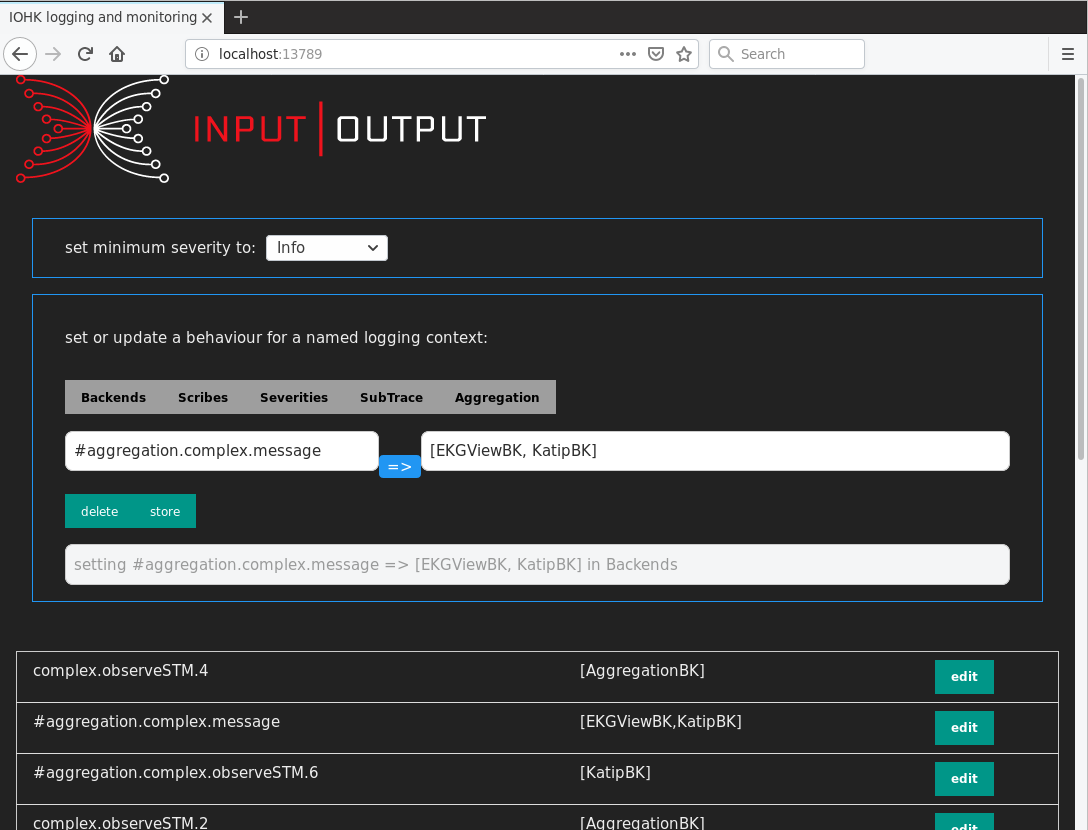
\includegraphics[scale=0.415]{ConfigEditor.pdf}
    }
    \caption{The configuration editor is listening on \emph{localhost} and can be accessed through a browser.
    At the top is the setting for the global minimum severity filter, that drops all messages that have a
    severity lower than this setting. Below are the settings for various behaviours of the logging system.
    }\label{fig:configeditor}
    \end{figure}
    
